%!TEX root =main.tex
\section{Upper bounding the distinguishing power}
\floris{
In this section we bound several class of GNNs by WL or WLL. Our key observations are the following: when GNNs do not incorporate self-features
then they are bounded by WWL, otherwise they are bounded by WL. Furthermore,
whenever $\mathbf{R}$ contains degree information, GNNs are one-step ahead
of WWL and WL.}

\tobdone{
Transition from the general GNN architecture using $\mathbf{N}$ in the previous section to the special cases. GNNs of the form~(\ref{eq:architecture}) below. Filip: how did you envisage this transition?}

We start by analysing the distinguishing power of GNN architectures of the form:
% We consider a GNN architecture which generalises commonly used GNN architectures. Given a labeled
% graph $(G,\pmb{\ell})$ with $G=(V,E)$, we denote by $\mathbf{F}^{(t)}$ the feature matrix assigning to each vertex $v\in V$ a feature vector $\mathbf{F}_{v\bullet}$. In layer $t$ of the the GNN architecture, $\mathbf{F}^{(t)}$ is updated as follows:
\begin{equation}
\mathbf{F}^{(t)}:=\sigma\left(\mathbf{F}^{(t-1)}\mathbf{W}_1^{(t-1)}+\mathbf{L}(\mathbf{A}+p\mathbf{I})\mathbf{R}\mathbf{F}^{(t-1)}\mathbf{W}_2^{(t-1)} + q\mathbf{B}^{(t-1)}\right), \label{eq:architecture}
\end{equation}
where $\mathbf{L}$ and $\mathbf{R}$ positive diagonal matrices, $p$ and $q$ are learnable parameters in $[0,1]$,  $\mathbf{W}_1^{(t-1)}$ and $\mathbf{W}_2^{(t-1)}$  are learnable weight matrices, $\mathbf{B}^{(t-1)}$ is a bias matrix with all the same rows, and finally, $\sigma$ is a non-linear activation function such as sign or ReLU. It should be clear that by choosing 
$\mathbf{L}$, $\mathbf{R}$, $p$ and $q$  in an appropriate way, one can obtain all GNN architectures mentioned so far.

Although it is possible to upper bound the distinguishing power of GNNs of the form~(\ref{eq:architecture}) in full generality\footnote{To this aim it suffices to incorporate the entries in the matrices $\mathbf{L}$ and $\mathbf{R}$ in the labelings and use WL on this extended labeling.}, we make the following additional assumptions on the matrices $\mathbf{L}$ and $\mathbf{R}$, motivated by the specific instantiations of $\mathbf{L}$ and $\mathbf{R}$ in GNNs found in the literature.

Let us denote by $\pmb{\ell}^L:V\to \Rb$ the vertex labeling defined by $\pmb{\ell}^L(v):=\mathbf{L}_{vv}$ and by $\pmb{\ell}^R:V\to \Rb$ the vertex labeling defined by 
$\pmb{\ell}^R(v):=\mathbf{R}_{vv}$ for all $v\in V$. We say that GNNs of the form~(\ref{eq:architecture}) are \textit{degree-determined} if, for any given  labeled graph $(G,\pmb{\ell})$, if $d_v=d_w$ then $\pmb{\ell}^L_v=\pmb{\ell}^L_w$ and $\pmb{\ell}^R_v=\pmb{\ell}^R_w$ hold. In other words,
the entries on the diagonals in $\mathbf{L}$ and $\mathbf{R}$ only depend on the degree of vertices.
We denote by ${\cal C}_{\textsl{deg}}$ the class of GNN architectures of the form~(\ref{eq:architecture}) that are degree-determined.

In ${\cal C}_{\textsl{deg}}$ we further zoom in on some special GNNs.
In particular, we also consider the case when  $\pmb{\ell}^R$ is a 
\textit{constant} labeling. We say that a  GNN of the form~(\ref{eq:architecture}) is \textit{constant on the right} if
it belongs to ${\cal C}_{\textsl{deg}}$ and
$\pmb{\ell}^R_v=\pmb{\ell}^R_w$ for all $v,w\in V$. In other words, the entries on the diagonal $\mathbf{R}$ are all the same, i.e., $\mathbf{R}$ is (a multiple of the) identity matrix $\mathbf{I}$.
We denote by ${\cal C}_{\textsl{cst}}$ the class of GNN architectures of the form~(\ref{eq:architecture}) that are constant on the right. By definition,
${\cal C}_{\textsl{cst}}\subseteq {\cal C}_{\textsl{deg}}$.

It is easily verified that all GNN architectures
mentioned earlier reside in the class ${\cal C}_{\textsl{deg}}$ and those
in which $\mathbf{R}=\mathbf{I}$  belong to 
the smaller class ${\cal C}_{\textsl{cst}}$.


With regards to their distinguishing power, GNNs in ${\cal C}_{\textsl{deg}}$
are still bounded by WL but with a factor of $1$. That is, they are one step ahead of WL. This is because  the diagonal entries in $\mathbf{R}$ carry information about degrees which are only determined during the first step of the WL algorithm. In contrast, GNNs in ${\cal C}_{\textsl{cst}}$ are bounded by WL, without any additional factor. This holds, even when $\mathbf{L}$ contains degree information. It shows an asymmetry between $\mathbf{L}$ and $\mathbf{R}$
and in terms of distinguishing power, $\mathbf{L}$ can be omitted from GNN architectures. \floris{There may be other arguments, perhaps spectral-based, that are in favour of keeping $\mathbf{L}$? Don't know.}

\tobdone{In the upper bound proofs it is always assumed that $\pmb{\ell}\sqsubseteq \mathbf{F}^{(0)}$. This seems something that needs to be incorporated when we say that one class is weaker than another one? There is also a comment wrt initial labeling below.}
\begin{proposition}\label{prop:boundconstantR}
The class ${\cal C}_{\textsl{cst}}$  is bounded by WL.
% Let $(G,\pmb{\ell})$ be a labeled graph and assume that $\pmb{\ell}\sqsubseteq\mathbf{F}^{(0)}$.
%  % for some $k\geq 0$.
% Then, GNN architectures of the form~(\ref{eq:architecture}) with constant $\pmb{\ell}^R$ are bounded by WL on $(G,\pmb{\ell})$.
\end{proposition}
\begin{proof}
We recall that ${\cal C}_{\textsl{WL}}$ just consists of the WL-algorithm, generating vertex labelings $\pmb{\ell}{}^{(0)}:=\pmb{\ell},\pmb{\ell}^{(1)},\ldots, \pmb{\ell}^{(k)}$. We show that for any GNN in 
${\cal C}_{\textsl{cst}}$, if we denote by
 $\mathbf{F}^{(0)},\mathbf{F}^{(1)},\ldots, \mathbf{F}^{(k)}$ the features
 computed in the different layers, then it holds that $\pmb{\ell}{}^{(t)}\sqsubseteq \mathbf{F}^{(t)}$ for any $t$. 

We verify this by induction on the number of iterations. For $t=0$, we have, by assumption, that 
$\pmb{\ell}\sqsubseteq \mathbf{F}^{(0)}$. Hence, the hypothesis holds for the base case.
% \pmb{\ell}{}^{(1)}\sqsubseteq
% Clearly,
%
% $\hat{\pmb{\ell}}{}^{(0)}\sqsubseteq \pmb{\ell}$ and hence also
% $\hat{\pmb{\ell}}{}^{(0)}\sqsubseteq\mathbf{F}^{(0)}$.
 We next assume that the induction hypothesis holds for all layers smaller than $t$ and consider layer $t$. More specifically, we assume that 
 $\pmb{\ell}^{(t-1)}\sqsubseteq \mathbf{F}^{(t-1)}$ and
 % For GNN architectures with non-constant $\pmb{\ell}^R$ (but degree-determined), we assume that $\pmb{\ell}^{(t+1)}\sqsubseteq \mathbf{F}^{(t)}$.
we need to show that 
$\pmb{\ell}{}^{(t)}_v=\pmb{\ell}{}^{(t)}_w$ implies that $\mathbf{F}^{(t)}_{v\bullet}=\mathbf{F}^{(t)}_{w\bullet}$. By definition,
$\pmb{\ell}{}^{(t)}_v=\pmb{\ell}{}^{(t)}_w$ implies
$\pmb{\ell}{}^{(t-1)}_v=\pmb{\ell}{}^{(t-1)}_w$ and 
$$
\ldbl \pmb{\ell}{}^{(t-1)}_u \st u \in N_G(v) \rdbl=
 \ldbl \pmb{\ell}{}^{(t-1)}_u \st u \in N_G(w) \rdbl.$$
 In other words, there exists a bijection between $N_G(v)$ and $N_G(w)$ such that for each $u\in N_G(v)$ and corresponding $u'\in N_G(w)$, $\pmb{\ell}{}^{(t-1)}_u=\pmb{\ell}{}^{(t-1)}_{u'}$. This bijection also implies 
 that $d_v=d_w$ and hence $\pmb{\ell}^L_{v}=\pmb{\ell}^L_{w}$ since we consider the class ${\cal C}_{\textsl{cst}}$. That is,
 $\mathbf{L}_{vv}=\mathbf{L}_{ww}$. Furthermore, we recall that in this class of GNNs, $\mathbf{R}_{uu}=\mathbf{R}_{u'u'}$ for any $u,u'\in V$. From the induction hypothesis we further know that 
 $\mathbf{F}^{(t-1)}_{v\bullet}=\mathbf{F}^{(t-1)}_{w\bullet}$ and 
 $\mathbf{F}^{(t-1)}_{u\bullet}=\mathbf{F}^{(t-1)}_{u'\bullet}$ for  every $u\in N_G(v)$ and corresponding $u'\in N_G(w)$.
%
%   Furthermore,
% since $\pmb{\ell}{}^{(t)}\sqsubseteq \pmb{\ell}{}^{(t-1)}\sqsubseteq \cdots\sqsubseteq \pmb{\ell}{}^{(1)}\sqsubseteq \pmb{\ell}{}^{(0)}$, we have that
%  $\pmb{\ell}{}^{(0)}_u=\pmb{\ell}{}^{(0)}_{u'}$ for every $u\in N_G(v)$ and corresponding
%  $u'\in N_G(w)$. In particular, we have that $d_u=d_{u'}$ and thus also $\mathbf{L}_{uu}=\mathbf{L}_{u'u'}$ and
%
%  this implies that
%  $\hat{\pmb{\ell}}{}^{(0)}_v=\hat{\pmb{\ell}}{}^{(0)}_w$ and that there is a bijection $b:N_G(v)\to N_G(w):u\mapsto u'$ such that $\hat{\pmb{\ell}}{}^{(t)}_u=\hat{\pmb{\ell}}{}^{(t)}_{u'}$ and hence also
%  $\hat{\pmb{\ell}}{}^{(0)}_u=\hat{\pmb{\ell}}{}^{(0)}_{u'}$. From the definition of $\hat{\pmb{\ell}}{}^{(0)}$, $\hat{\pmb{\ell}}{}^{(0)}_v=\hat{\pmb{\ell}}{}^{(0)}_w$ implies that
%  $\mathbf{L}_{vv}=\mathbf{L}_{ww}$ and
%  $\mathbf{R}_{vv}=\mathbf{R}_{ww}$. Similarly, for every $u\in N_G(v)$ and corresponding $u'\in N_G(w)$,
% $\hat{\pmb{\ell}}{}^{(0)}_u=\hat{\pmb{\ell}}{}^{(0)}_{u'}$ implies that   $\mathbf{L}_{uu}=\mathbf{L}_{u'u'}$ and $\mathbf{R}_{uu}=\mathbf{R}_{u'u'}$. By the induction hypothesis we also have that
%  $\mathbf{F}^{(t)}_{v\bullet}=\mathbf{F}^{(t)}_{w\bullet}$, and for every $u\in N_G(v)$
%    and corresponding $u'\in N_G(w)$, $\mathbf{F}^{(t)}_{u\bullet}=\mathbf{F}^{(t)}_{u'\bullet}$.
  It now suffices to observe that
  \begin{align*}
	  \mathbf{F}^{(t)}_{v\bullet}&=\sigma\Biggl(\mathbf{F}^{(t-1)}_{v\bullet}\mathbf{W}_1^{(t-1)}+\mathbf{L}_{vv}\biggl(\Bigl(\sum_{u\in N_G(v)} \mathbf{R}_{uu}\mathbf{F}^{(t-1)}_{u\bullet}\Bigr)+p\mathbf{R}_{vv}\mathbf{F}^{(t-1)}_{v\bullet}\biggr)\mathbf{W}_2^{(t-1)}+ q\mathbf{B}^{(t-1)}_{v\bullet}\Biggr)\\
	 &=\sigma\Biggl(\mathbf{F}^{(t-1)}_{w\bullet}\mathbf{W}_1^{(t-1)}+\mathbf{L}_{ww}\biggl(\Bigl(\sum_{u\in N_G(w)} \mathbf{R}_{uu}\mathbf{F}^{(t-1)}_{u\bullet}\Bigr)+p\mathbf{R}_{ww}\mathbf{F}^{(t-1)}_{v\bullet}\biggr)\mathbf{W}_2^{(t-1)}+ q\mathbf{B}^{(t-1)}_{w\bullet}\Biggr) \end{align*}
as desired. We here additionally used that $\mathbf{B}^{(t-1)}$ is a matrix consisting of all the same rows and hence $\mathbf{B}^{(t-1)}_{v\bullet}=\mathbf{B}^{(t-1)}_{w\bullet}$ for any $v,w\in V$.
\end{proof}

For the class ${\cal C}_{\textsl{deg}}$ we obtain the following upper bound.
% When $\pmb{\ell}^R$ is not constant, but nevertheless degree-determined, we obtain the following upper bound.
\begin{proposition}\label{prop:boundnonconstantR}
	The class ${\cal C}_{\textsl{deg}}$ is bounded by WL, with a factor $1$.	
%
% Let $(G,\pmb{\ell})$ be a labeled graph and assume that $\pmb{\ell}\sqsubseteq\mathbf{F}^{(0)}$.
%  % for some $k\geq 0$.
% Then, GNN architectures of the form~(\ref{eq:architecture}) with non-constant $\pmb{\ell}^R$ are bounded by WL on $(G,\pmb{\ell}^{(1)})$.
\end{proposition}
\begin{proof}
The proof is almost the same as the previous proof. That is,
we show the upper bound by WL by induction on the number of iterations. For $t=0$, we have, by assumption, that 
$\pmb{\ell}\sqsubseteq \mathbf{F}^{(0)}$. Hence, since $\pmb{\ell}{}^{(1)}\sqsubseteq\pmb{\ell}$ we also have that $\pmb{\ell}{}^{(1)}\sqsubseteq\mathbf{F}^{(0)}$ and 
the induction hypothesis holds for the base case.
% \pmb{\ell}{}^{(1)}\sqsubseteq
% Clearly,
%
% $\hat{\pmb{\ell}}{}^{(0)}\sqsubseteq \pmb{\ell}$ and hence also
% $\hat{\pmb{\ell}}{}^{(0)}\sqsubseteq\mathbf{F}^{(0)}$.
 We next assume that the induction hypotheses holds for $t\geq 0$ and consider $t+1$. More specifically, we assume that 
 $\pmb{\ell}^{(t+1)}\sqsubseteq \mathbf{F}^{(t)}$ and
 % For GNN architectures with non-constant $\pmb{\ell}^R$ (but degree-determined), we assume that $\pmb{\ell}^{(t+1)}\sqsubseteq \mathbf{F}^{(t)}$.
we need to show that 
$\pmb{\ell}{}^{(t+2)}_v=\pmb{\ell}{}^{(t+2)}_w$ implies that $\mathbf{F}^{(t+1)}_{v\bullet}=\mathbf{F}^{(t+1)}_{w\bullet}$. By definition,
$\pmb{\ell}{}^{(t+2)}_v=\pmb{\ell}{}^{(t+2)}_w$ implies
$\pmb{\ell}{}^{(t+1)}_v=\pmb{\ell}{}^{(t+1)}_w$ and 
$$
\ldbl \pmb{\ell}{}^{(t+1)}_u \st u \in N_G(v) \rdbl=
 \ldbl \pmb{\ell}{}^{(t+1)}_u \st u \in N_G(w) \rdbl.$$
 In other words, there exists a bijection between $N_G(v)$ and $N_G(w)$ such that for each $u\in N_G(v)$ and corresponding $u'\in N_G(w)$, $\pmb{\ell}{}^{(t+1)}_u=\pmb{\ell}{}^{(t+1)}_{u'}$. 
  This bijection also implies that
 that $d_v=d_w$ and hence $\pmb{\ell}^L_{v}=\pmb{\ell}^L_{w}$ and $\pmb{\ell}^{R}_{v}=\pmb{\ell}^R_{w}$. That is,
 $\mathbf{L}_{vv}=\mathbf{L}_{ww}$ and $\mathbf{R}_{vv}=\mathbf{R}_{ww}$ hold.
We next argue in a different way as in the previous proof. We observe that
 $\pmb{\ell}{}^{(t+1)}\sqsubseteq \pmb{\ell}{}^{(t)}\sqsubseteq \cdots\sqsubseteq \pmb{\ell}{}^{(1)}$. Hence, we have that $\pmb{\ell}{}^{(t+1)}_u=\pmb{\ell}{}^{(t+1)}_{u'}$ implies 
 $\pmb{\ell}{}^{(1)}_u=\pmb{\ell}{}^{(1)}_{u'}$. We note that this implication was not guaranteed in the previous proof. Indeed, we can only infer that  $\pmb{\ell}{}^{(0)}_u=\pmb{\ell}{}^{(0)}_{u'}$ when $t=1$. 
In the current setting, we thus know that $d_{u}=d_{u'}$ for every $u\in N_G(v)$ and $u'\in N_G(w)$. We may thus infer that $\mathbf{R}_{uu}=\mathbf{R}_{u'u'}$ for every $u\in N_G(v)$ and corresponding $u'\in N_G(w)$.
 From the induction hypothesis we further know that 
 $\mathbf{F}^{(t)}_{v\bullet}=\mathbf{F}^{(t)}_{w\bullet}$ and 
 $\mathbf{F}^{(t)}_{u\bullet}=\mathbf{F}^{(t)}_{u'\bullet}$ for  every $u\in N_G(v)$ and corresponding $u'\in N_G(w)$.
%
%   Furthermore,
% since $\pmb{\ell}{}^{(t)}\sqsubseteq \pmb{\ell}{}^{(t-1)}\sqsubseteq \cdots\sqsubseteq \pmb{\ell}{}^{(1)}\sqsubseteq \pmb{\ell}{}^{(0)}$, we have that
%  $\pmb{\ell}{}^{(0)}_u=\pmb{\ell}{}^{(0)}_{u'}$ for every $u\in N_G(v)$ and corresponding
%  $u'\in N_G(w)$. In particular, we have that $d_u=d_{u'}$ and thus also $\mathbf{L}_{uu}=\mathbf{L}_{u'u'}$ and
%
%  this implies that
%  $\hat{\pmb{\ell}}{}^{(0)}_v=\hat{\pmb{\ell}}{}^{(0)}_w$ and that there is a bijection $b:N_G(v)\to N_G(w):u\mapsto u'$ such that $\hat{\pmb{\ell}}{}^{(t)}_u=\hat{\pmb{\ell}}{}^{(t)}_{u'}$ and hence also
%  $\hat{\pmb{\ell}}{}^{(0)}_u=\hat{\pmb{\ell}}{}^{(0)}_{u'}$. From the definition of $\hat{\pmb{\ell}}{}^{(0)}$, $\hat{\pmb{\ell}}{}^{(0)}_v=\hat{\pmb{\ell}}{}^{(0)}_w$ implies that
%  $\mathbf{L}_{vv}=\mathbf{L}_{ww}$ and
%  $\mathbf{R}_{vv}=\mathbf{R}_{ww}$. Similarly, for every $u\in N_G(v)$ and corresponding $u'\in N_G(w)$,
% $\hat{\pmb{\ell}}{}^{(0)}_u=\hat{\pmb{\ell}}{}^{(0)}_{u'}$ implies that   $\mathbf{L}_{uu}=\mathbf{L}_{u'u'}$ and $\mathbf{R}_{uu}=\mathbf{R}_{u'u'}$. By the induction hypothesis we also have that
%  $\mathbf{F}^{(t)}_{v\bullet}=\mathbf{F}^{(t)}_{w\bullet}$, and for every $u\in N_G(v)$
%    and corresponding $u'\in N_G(w)$, $\mathbf{F}^{(t)}_{u\bullet}=\mathbf{F}^{(t)}_{u'\bullet}$.
  It now suffices to observe that
  \begin{align*}
	  \mathbf{F}^{(t+1)}_{v\bullet}&=\sigma\Biggl(\mathbf{F}^{(t)}_{v\bullet}\mathbf{W}_1^{(t)}+\mathbf{L}_{vv}\biggl(\Bigl(\sum_{u\in N_G(v)} \mathbf{R}_{uu}\mathbf{F}^{(t)}_{u\bullet}\Bigr)+p\mathbf{R}_{vv}\mathbf{F}^{(t)}_{v\bullet}\biggr)\mathbf{W}^{(t)}+ q\mathbf{J}_{v\bullet}\Biggr)\\
	 & =\sigma\Biggl(\mathbf{F}^{(t)}_{w\bullet}\mathbf{W}_1^{(t)}+\mathbf{L}_{ww}\biggl(\Bigl(\!\!\sum_{u'\in N_G(w)}\!\! \mathbf{R}_{u'u'}\mathbf{F}^{(t)}_{u'\bullet}\Bigr)+p\mathbf{R}_{ww}\mathbf{F}^{(t)}_{w\bullet}\biggr)\mathbf{W}^{(t)}+ q\mathbf{J}_{w\bullet}\Biggr)\\
	  &=\mathbf{F}^{(t+1)}_{w\bullet},
\end{align*}
as desired.
\end{proof}

In other words, we have that ${\cal C}_{\textsl{deg}}\sqsubseteq {\cal C}_{\textsl{WL}}$ with constant factor $1$, and ${\cal C}_{\textsl{cst}}\sqsubseteq {\cal C}_{\textsl{WL}}$, without any factor.
Whenever ${\cal C}\sqsubseteq {\cal C}'$ without any factor, then clearly
also ${\cal C}\sqsubseteq {\cal C}'$, with any constant factor. The converse does not hold, in general, as illustrated by the following example.
%
%
% when a class of GNNs is bounded by WL, without any
% It should be clear that GNNs of the form~(\ref{eq:architecture}) which are bounded by WL on $(G,\pmb{\ell})$ are also bounded by WL on $(G,\pmb{\ell}{}^{(1)})$. The converse is not true, as is illustrated by the following example.
\openprob{Is there a simpler example for the one below?}
\begin{example}\label{ex2}\normalfont
	We consider NA-GNN+ architecture~\cite{kipf-loose} in which $\pmb{\ell}^R$ is non-constant and thus Proposition~\ref{prop:boundnonconstantR} applies.
Consider the labeled graph $(G,\pmb{\ell})$ (\raisebox{-2ex}{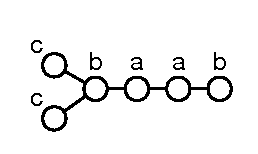
\includegraphics[height=1cm]{graph1}}) with 
vertex labeling  $\pmb{\ell}_{v_1}=\pmb{\ell}_{v_2}=c$,
$\pmb{\ell}_{v_3}=\pmb{\ell}_{v_6}=b$ and $\pmb{\ell}_{v_4}=\pmb{\ell}_{v_5}=a$, and adjacency and degree matrix 
$$
\mathbf{A}:=\begin{bmatrix}
0 & 0 & 1 & 0 & 0 & 0\\
0 & 0 & 1 & 0 & 0 & 0\\
1 & 1 & 0 & 1 & 0 & 0\\
0 & 0 & 1 & 0 & 1 & 0\\
0 & 0 & 0 & 1 & 0 & 1\\
0 & 0 & 0 & 0 & 1 & 0
\end{bmatrix}\text{ and } 
\mathbf{D}:=
\begin{bmatrix}
1 & 0 & 0 & 0 & 0 & 0\\
0 & 1 & 0 & 0 & 0 & 0\\
0 & 0 & 3 & 0 & 0 & 0\\
0 & 0 & 0 & 2 & 0 & 0\\
0 & 0 & 0 & 0 & 2 & 0\\
0 & 0 & 0 & 0 & 0 & 1
\end{bmatrix},
$$
respectively. 
We consider $\mathbf{F}^{(1)}:=\sigma(\tilde{\mathbf{D}}^{-1/2}(\mathbf{A}+\mathbf{I})\tilde{\mathbf{D}}^{-1/2}\mathbf{F}^{(0)}\mathbf{W}^{(0)})$ with  $
\mathbf{F}^{(0)}=
\left[\begin{smallmatrix}
1 & 0 & 0\\
1 & 0 & 0\\
0 & 1 & 0\\
0 & 0 & 1\\
0 & 0 & 1\\
0 & 1 & 0\\
\end{smallmatrix}\right]
$ and choose $\mathbf{W}^{(0)}=\left[\begin{smallmatrix}
1 & 0 & 0\\
0 & 1 & 0\\
0 & 0 & 1
\end{smallmatrix}\right]$. 
We remark that $\pmb{\ell}^{(0)}:=\pmb{\ell}\equiv \mathbf{F}^{(0)}$.
It can be verified that
$$
\mathbf{F}^{(1)}=\sigma\left(\begin{bmatrix}
\frac{1}{2} & \frac{1}{2\sqrt{2}}& 0\\
\frac{1}{2} & \frac{1}{2\sqrt{2}}& 0\\
\frac{1}{2\sqrt{2}} & \frac{1}{4}& \frac{1}{
2\sqrt{3}}\\
0 & \frac{1}{2\sqrt{3}}& \frac{2}{
3}\\
0 & \frac{1}{\sqrt{6}}& \frac{2}{
3}\\
0 & \frac{1}{2}& \frac{1}{
\sqrt{6}}
\end{bmatrix}\right).
$$
Suppose that $\sigma$ is the ReLU activation function. Then, we observe that
$\mathbf{F}^{(1)}_{v_4\bullet}\neq \mathbf{F}^{(1)}_{v_5\bullet}$. 
We note, however, that $\pmb{\ell}^{(1)}_{v_4}=(a,\{a,b\})=\pmb{\ell}^{(1)}_{v_5}$.
Hence, $\pmb{\ell}^{(1)}\not\sqsubseteq \mathbf{F}^{(1)}$ and this architecture is not bounded by WL, without the additional constant factor $1$.
In accordance with Proposition~\ref{prop:boundnonconstantR}, one can verify
that $\pmb{\ell}^{(2)}\sqsubseteq \mathbf{F}^{(1)}$.
 % We know, however, that it is bounded by WL on $(G,\pmb{\ell}{}^{(1)})$.
\qed
% It can, however, be verified that $\pmb{\ell}^{(2)}\sqsubseteq \mathbf{F}^{(1)}$.
% \todo{The latter inclusion needs to be verified}\qed
\end{example}



%
%
%
% We conclude this section by observing that previous propositions generalise as follows.
% \begin{corollary}
% \begin{itemize}
% \item[(a)]Let $(G,\pmb{\ell})$ be a labeled graph and assume that $\pmb{\ell}^{(k)}\sqsubseteq\mathbf{F}^{(0)}$ for some $k\geq 0$.
% Then, GNN architectures of the form~(\ref{eq:architecture}) with constant $\pmb{\ell}^R$ are bounded by WL on $(G,\pmb{\ell}^{(k)})$.
% \item[(b)] Let $(G,\pmb{\ell})$ be a labeled graph and assume that $\pmb{\ell}^{(k)}\sqsubseteq\mathbf{F}^{(0)}$ for some $k\geq 0$.
% Then, GNN architectures of the form~(\ref{eq:architecture}) with non-constant $\pmb{\ell}^R$ are bounded by WL on $(G,\pmb{\ell}^{(k+1)})$.
% \end{itemize}
% \end{corollary}
% %  $\pmb{\ell}^{(k)}\sqsubseteq\hat{\pmb{\ell}}$
% % and $\pmb{\ell}^{(k)}\sqsubseteq\hat{\pmb{\ell}}$ and $$
% %
% % Remark: iterated degrees...
% % More generally, we have the following property.
% % \begin{corollary}\label{cor:augmented}
% % If $\pmb{\ell}^{(k)}\sqsubseteq\hat{\pmb{\ell}}$ holds, then the GNN architecture~(\ref{eq:architecture})  is bounded by 1-WL, starting from $\pmb{\ell}^{(k)}$.
% % \end{corollary}
% % Intuitively, this implies that the GNN architecture is $k$-steps ahead of the 1-WL algorithm.
% % More precisely, $\pmb{\ell}^{(t)}\sqsubseteq \mathbf{F}^{(t-k)}$ for $t\geq k$.
% \begin{proof}
% \tobdone{Proof.}
% % 	For (a)~, if 	$\pmb{\ell}^{(k)}\sqsubseteq\hat{\pmb{\ell}}$ holds, then also
% % $\pmb{\ell}^{(k+t)}\sqsubseteq\hat{\pmb{\ell}}{}^{(t)}$ holds for any $t\geq 0$. Hence,
% % $\pmb{\ell}^{(k+t)}\sqsubseteq \mathbf{F}^{(t)}$ or $\pmb{\ell}^{(k)}\sqsubseteq\mathbf{F}^{(t-k)}$ by Theorem~\ref{thm:generalbound}.
% % For (b)~, it is easily verified that the proof of Corollary~\ref{cor:weak} can be generalized to this setting.
% \end{proof}

\openprob{Perhaps we could point out that the one-step advantage of 
GNNs in ${\cal C}_{\textsl{deg}}$ over GNNs in ${\cal C}_{\textsl{cst}}$
can be easily overcome, at least theoretically. How? We just kickstart
GNNs in  ${\cal C}_{\textsl{cst}}$ with a labeling $\pmb{\ell}$ that contains
degree information, e.g., $\hat{\pmb{\ell}}_v=(\pmb{\ell},d_v)$ for each $v\in V$. The current definition of how we compare two classes of GNNs may need some
revision, since in that definition the same $\pmb{\ell}$ is assumed. More generally, one can start running GNNs from labelings that incorporate information
which WL only detects after a number of iterations. The reason that I want to do this is because a paper I found on  Graph Feature Networks (GFNs)~\cite{chen2019powerful}. In such networks, the initial feature vectors $\mathbf{F}^{(0)}$ are expanded to $\hat{\mathbf{F}}{}^{(0)}:=[\mathbf{d},\mathbf{F}^{(0)},\mathbf{N}\mathbf{F}^{(0)},\ldots,\mathbf{N}^k\mathbf{F}^{(0)}]$ with $\mathbf{N}=\tilde{\mathbf{D}}^{-1/2}(\mathbf{A}+p\mathbf{I})\tilde{\mathbf{D}}^{-1/2}$ and 
$\mathbf{F}^{(1)}:=\sigma(\hat{\mathbf{F}}{}^{(0)}\mathbf{W}^{(0)})$ and for $t>1$: $\mathbf{F}^{(t)}:=\sigma(\mathbf{F}{}^{(t-1)}\mathbf{W}^{(t-1)})$.
It needs further investigation what precisely can be said here. The paper seems to say that in this way less layers are needed. We may want to make this precise.
}

As previously mentioned, some of the GNN architectures do not incorporate the features of the vertices themselves in each layer. We next show that such GNNs are bounded in their distinguishing power by WWL. More specifically, let ${\cal C}_{\textsl{noself}}$ be the class of GNN architectures of the form ~(\ref{eq:architecture}) such that in each layer $\mathbf{W}_1^{(t)}$ is absent (i.e., it is always set to $\mathbf{O}$) and $p=0$ (i.e., the identity matrix $\mathbf{I}$ is ignored).

To state our result we need a notion of labeled graphs which are consistent with degree information. More specifically, these are labeled graphs $(G,\pmb{\ell})$ such that $d_v=d_w\Rightarrow \pmb{\ell}_v=\pmb{\ell}_w$. In other words, vertices with the same degree should not be labeled differently.

\begin{proposition}
(a)~The class  ${\cal C}_{\textsl{noself}}\cap {\cal C}_{\textsl{cst}}$ is bounded by WWL (with no additional factor). (b)~
The class ${\cal C}_{\textsl{noself}}\cap {\cal C}_{\textsl{deg}}$ is bounded by WWL with a factor $1$ on labeled graphs $(G,\pmb{\ell})$ consistent with degree information.
\end{proposition}
\begin{proof}
In the proof we use $\pmb{\mu}$ for $\pmb{\ell}$ to make the distinction between WL and WWL clear.

(a)~We show the upper bound by WWL by induction on the number of iterations. For $t=0$, we have, by assumption, that 
$\pmb{\mu}\sqsubseteq \mathbf{F}^{(0)}$. 
% Since we consider labeled graphs which are consistent with degree information, and $\pmb{\mu}^{(1)}_v=\pmb{\mu}^{(1)}_w$
% implies $d_v=d_w$, we also h
We next assume that the induction hypothesis holds for $t\geq 0$ and consider $t+1$. We need to show that 
$\pmb{\mu}{}^{(t+1)}_v=\pmb{\mu}{}^{(t+1)}_w$ implies that $\mathbf{F}^{(t+1)}_{v\bullet}=\mathbf{F}^{(t+1)}_{w\bullet}$. By definition,
$\pmb{\mu}^{(t+1)}_v=\pmb{\mu}{}^{(t+1)}_w$ implies
$$
\ldbl \pmb{\mu}{}^{(t)}_u \st u \in N_G(v) \rdbl=
 \ldbl \pmb{\mu}{}^{(t)}_u \st u \in N_G(w) \rdbl.$$
We remark that this implies that $d_v=d_w$. Since our GNNs belong to ${\cal C}_{\textsl{cst}}$, this in turn implies that $\mathbf{L}_{vv}=\mathbf{L}_{ww}$.
In addition, $\mathbf{R}_{uu}=\mathbf{R}_{u'u'}$ for all $u,u'\in V$.
%
% It is readily verified that $\hat{\pmb{\mu}}{}^{(t)}\sqsubseteq \hat{\pmb{\mu}}{}^{(t-1)}\sqsubseteq \cdots\sqsubseteq \hat{\pmb{\mu}}{}^{(1)}$ for $t>1$. We remark that in general, $\hat{\pmb{\mu}}{}^{(1)}\not\sqsubseteq \hat{\pmb{\mu}}{}^{(0)}$.
Furthermore, there is a bijection between $N_G(v)$ and $N_G(w)$ such that for each $u\in N_G(v)$ and corresponding $u'\in N_G(w)$, $\pmb{\mu}{}^{(t)}_u=\pmb{\mu}{}^{(t)}_{u'}$.
% %  and hence also
% %  $\pmb{\mu}{}^{(1)}_u=\pmb{\mu}{}^{(1)}_{u'}$.
% % %
% %
% % Since $\h\pmb{\mu}}{}^{(0)}\sqsubseteq \pmb{\mu}^{(1)}$, this implies that for every $u\in N_G(v)$ and corresponding $u'\in N_G(w)$,  $\pmb{\mu}{}^{(1)}_u=\pmb{\mu}{}^{(1)}_{u'}$.
% % By our assumption on $\pmb{\mu}^{(1)}$, this implies that
% $\mathbf{L}_{uu}=\mathbf{L}_{u'u'}$ and $\mathbf{R}_{uu}=\mathbf{R}_{u'u'}$. Similarly,
% $\hat{\pmb{\mu}}{}^{(t+1)}_v=\hat{\pmb{\mu}}{}^{(t+1)}_w$  implies
% $\pmb{\mu}{}^{(1)}_v=\pmb{\mu}{}^{(1)}_{w}$ and thus also $\mathbf{L}_{vv}=\mathbf{L}_{ww}$.
By the induction hypothesis we also have that for  every $u\in N_G(v)$
   and corresponding $u'\in N_G(w)$, $\mathbf{F}^{(t)}_{u\bullet}=\mathbf{F}^{(t)}_{u'\bullet}$. It now suffices to observe that
  \begin{align*}
  \mathbf{F}^{(t+1)}_{v\bullet}&=\sigma\Biggl(\mathbf{L}_{vv}\Bigl(\sum_{u\in N_G(v)} \mathbf{R}_{uu}\mathbf{F}^{(t)}_{u\bullet}\Bigr)\mathbf{W}^{(t)}+ q\mathbf{B}^{(t)}_{v\bullet}\Biggr)\\
	 & =\sigma\Biggl(\mathbf{L}_{ww}\Bigl(\!\!\sum_{u'\in N_G(w)}\!\! \mathbf{R}_{u'u'}\mathbf{F}^{(t)}_{u'\bullet}\Bigr)\mathbf{W}^{(t)}+ q\mathbf{B}^{(t)}_{w\bullet}\Biggr)\\
	  &=\mathbf{F}^{(t+1)}_{w\bullet},
\end{align*}
as desired.


(b)~We show the upper bound by WWL by induction on the number of iterations. For $t=0$, we have, as before that $\pmb{\mu}\sqsubseteq \mathbf{F}^{(0)}$. 
We remark, however, that in general $\pmb{\mu}^{(1)}\not\sqsubseteq\pmb{\mu}$.
It is here that the restriction on labeled graphs come into play. More precisely,
$\pmb{\mu}^{(1)}_v=\pmb{\mu}^{(1)}_w$ implies that $d_v=d_w$. Since $(G,\pmb{\mu})$ is consistent with degree information, $d_v=d_w$ implies
$\pmb{\mu}_v=\pmb{\mu}_w$. So, on such graphs, $\pmb{\mu}^{(1)}\sqsubseteq\pmb{\mu}\sqsubseteq\mathbf{F}^{(0)}$.

% Since we consider labeled graphs which are consistent with degree information, and $\pmb{\mu}^{(1)}_v=\pmb{\mu}^{(1)}_w$
% implies $d_v=d_w$, we also h
We next assume that the induction hypothesis holds for $t\geq 0$ and consider $t+1$. We need to show that 
$\pmb{\mu}{}^{(t+2)}_v=\pmb{\mu}{}^{(t+2)}_w$ implies that $\mathbf{F}^{(t+1)}_{v\bullet}=\mathbf{F}^{(t+1)}_{w\bullet}$. By definition,
$\pmb{\mu}^{(t+2)}_v=\pmb{\mu}{}^{(t+2)}_w$ implies
$$
\ldbl \pmb{\mu}{}^{(t+1)}_u \st u \in N_G(v) \rdbl=
 \ldbl \pmb{\mu}{}^{(t+1)}_u \st u \in N_G(w) \rdbl.$$
We remark that this implies that $d_v=d_w$. Since our GNNs belong to ${\cal C}_{\textsl{deg}}$, this in turn implies that $\mathbf{L}_{vv}=\mathbf{L}_{ww}$.
%
% It is readily verified that $\hat{\pmb{\mu}}{}^{(t)}\sqsubseteq \hat{\pmb{\mu}}{}^{(t-1)}\sqsubseteq \cdots\sqsubseteq \hat{\pmb{\mu}}{}^{(1)}$ for $t>1$. We remark that in general, $\hat{\pmb{\mu}}{}^{(1)}\not\sqsubseteq \hat{\pmb{\mu}}{}^{(0)}$.
Furthermore, there is a bijection between $N_G(v)$ and $N_G(w)$ such that
for every $u\in N_G(v)$ and $u'\in N_G(w)$, $\pmb{\mu}{}^{(t+1)}_u=\pmb{\mu}{}^{(t+1)}_{u'}$. This in turn implies that
$d_u=d_{u'}$ for every $u\in N_G(v)$ and corresponding $u'\in N_G(w)$. We note that this holds because $t+1\geq 1$. Since our GNNs belong to ${\cal C}_{\textsl{deg}}$, we have that $\mathbf{R}_{uu}=\mathbf{R}_{u'u'}$ for every
$u\in N_G(v)$ and corresponding $u'\in N_G(w)$. 
% %  and hence also
% %  $\pmb{\mu}{}^{(1)}_u=\pmb{\mu}{}^{(1)}_{u'}$.
% % %
% %
% % Since $\h\pmb{\mu}}{}^{(0)}\sqsubseteq \pmb{\mu}^{(1)}$, this implies that for every $u\in N_G(v)$ and corresponding $u'\in N_G(w)$,  $\pmb{\mu}{}^{(1)}_u=\pmb{\mu}{}^{(1)}_{u'}$.
% % By our assumption on $\pmb{\mu}^{(1)}$, this implies that
% $\mathbf{L}_{uu}=\mathbf{L}_{u'u'}$ and $\mathbf{R}_{uu}=\mathbf{R}_{u'u'}$. Similarly,
% $\hat{\pmb{\mu}}{}^{(t+1)}_v=\hat{\pmb{\mu}}{}^{(t+1)}_w$  implies
% $\pmb{\mu}{}^{(1)}_v=\pmb{\mu}{}^{(1)}_{w}$ and thus also $\mathbf{L}_{vv}=\mathbf{L}_{ww}$.
By the induction hypothesis we also for every $u\in N_G(v)$
   and corresponding $u'\in N_G(w)$, $\mathbf{F}^{(t)}_{u\bullet}=\mathbf{F}^{(t)}_{u'\bullet}$. It now suffices to observe that
  \begin{align*}
  \mathbf{F}^{(t+1)}_{v\bullet}&=\sigma\Biggl(\mathbf{L}_{vv}\Bigl(\sum_{u\in N_G(v)} \mathbf{R}_{uu}\mathbf{F}^{(t)}_{u\bullet}\Bigr)\mathbf{W}^{(t)}+ q\mathbf{B}^{(t)}_{v\bullet}\Biggr)\\
	 & =\sigma\Biggl(\mathbf{L}_{ww}\Bigl(\!\!\sum_{u'\in N_G(w)}\!\! \mathbf{R}_{u'u'}\mathbf{F}^{(t)}_{u'\bullet}\Bigr)\mathbf{W}^{(t)}+ q\mathbf{B}^{(t)}_{w\bullet}\Biggr)\\
	  &=\mathbf{F}^{(t+1)}_{w\bullet},
\end{align*}
as desired.
\end{proof}

\openprob{I do not know whether the assumption on the initial labeling being consistent with degree information can be dropped in (b).}

\tobdone{Show example for WWL bounded with factor 1 but not bounded by WWL, no factor.}

\tobdone{Show example WL vs WLL bounded.}

\floris{I would like to make a connection with the work by Grohe. Note that WWL on unlabeled graphs corresponds to WL (Grohe paper). The above upper bounds using WWL can thus be seen as a generalisation of their unlabeled case to the labeled case. We recover the WWL (and thus WL) upper bound of $\sigma(\mathbf{A}\mathbf{F}^{(t-1)}\mathbf{W}^{(t-1)}-\mathbf{J})$ in their paper.}



% Intuitively, when $\pmb{\ell}^{(k)}\sqsubseteq\hat{\pmb{\ell}}$ holds for any labeled graph $(G,\pmb{\ell})$, then this implies that the entries in $\mathbf{L}$ and $\mathbf{R}$ are functionally determined by the so-called \textit{$k$-iterated degrees} of vertices. The $k$-iterated degree of a vertex $v$ is the label assigned by $k$-steps of  WL on the uniformily labeled graph $(G,\pmb{a})$ in which every vertex is assigned the label $a$.
% Similarly, $\pmb{\ell}^{(k')}_v=\pmb{\ell}^{(0)}_w\Rightarrow \mathbf{R}_{vv}=\mathbf{R}_{ww}$ implies that the entries in $\mathbf{R}$ are functionally determined by the $k'$-iterated degrees of vertices. We illustrate this by the following example.
% \begin{example}
% 	\floris{Show example for say, $k=2$, and $k=2$ and $k'=1$, if we think this is interesting.}
% \end{example}
